\documentclass[a4paper,12pt]{article} 

%%% Работа с русским языком
\usepackage{cmap}                           % поиск в PDF
\usepackage{mathtext} 			 	       % русские буквы в формулах
\usepackage[T2A]{fontenc}               % кодировка
\usepackage[utf8]{inputenc}              % кодировка исходного текста
\usepackage{siunitx}
\usepackage[english,russian]{babel}  % локализация и переносы
\usepackage[left=2cm,right=2cm,
    top=2cm,bottom=3cm,bindingoffset=0cm]{geometry}
\usepackage{wrapfig}
\usepackage{gensymb}
\usepackage{textcomp}
\usepackage{multirow}
\usepackage{pgfplots}
\usepackage{amsmath,amsfonts,amssymb,amsthm,mathtools} % AMS
\usepackage{euscript}	 % Шрифт Евклид
\usepackage{mathrsfs} % Красивый матшрифт
\usepackage{graphicx}%Вставка картинок правильная
\usepackage{float}%"Плавающие" картинки
\usepackage{wrapfig}%Обтекание фигур (таблиц, картинок и прочего)
\title{Лабораторная работа 1.3

Эффект Рамзауэра}
\author{Кагарманов Радмир Б01-102}
\date{4 декабря 2023 г.}

\begin{document}
\maketitle
\thispagestyle{empty}
\newpage
\setcounter{page}{1}

\paragraph{Цель работы:} исследовать энергетическую зависимость вероятности рассеяния электронов атомами инертного газа; определить энергии электронов, при которых наблюдается <<просветление>> газа; и оценить размер его электронной оболочки.

\paragraph{Теория\\}
Решим одномерное уравнение Шредингера для частицы, налетающей на потенциальную яму.

\begin{equation*}
U = 
 \begin{cases}
   0 &\text{, $x < 0$}\\
   -U_0 &\text{, $0<x<l$}\\
   0 &\text{, $x > l$}
 \end{cases}
\end{equation*}

В силу произвольности падающего потока частиц, удобно отнормировать его таким образом, чтобы $A$ была коэффициентом отражения, а $B$ - коэффициентом прохождения. Тогда решение для волновой функции надо искать в виде:

\begin{equation*}
\psi = 
 \begin{cases}
   e^{ik_1 x} + Ae^{-ik_1 x} &\text{, $x < 0$}\\
   C_1 e^{ik_2 x} + C_2 e^{-ik_2 x} &\text{, $0<x<l$}\\
   Be^{ik_1 x} &\text{, $x > l$}
 \end{cases}
\end{equation*}

Где $k_1^2 = \frac{2mE}{\hbar^2}$, $k_2^2 = \frac{2m(E + U_0)}{\hbar^2}$.

Из требований непрерывности и гладкости при $x=0$ и $x=l$ получаем систему уравнений и можем найти $B$.

\begin{equation}
    B=\frac{4k_1 k_2 e^{-ik_1 l}}{(k_1 + k_2)^2 e^{-ik_2 l} - (k_1 - k_2)^2 e^{ik_2 l}}
\end{equation}

Коэффициент прохождения над ямой:

\begin{equation}
    D = |B|^2
\end{equation}

После арифметических преобразований получаем:

\begin{equation}
    D=\frac{1}{1 + \frac{1}{4}(\sqrt{\frac{E}{E+U_0}} - \sqrt{\frac{E+U_0}{E}})^2 sin^2(\sqrt{E + U_0}[эВ]\frac{l[\textup{~\AA}]}{1.95})}
\end{equation}

Условие <<просветления>>: $\sqrt{E + U_0}[эВ]\frac{l[\textup{~\AA}]}{1.95} = \pi n$, условие <<затемнения>>: $\sqrt{E + U_0}[эВ]\frac{l[\textup{~\AA}]}{1.95} = \pi n + \frac{\pi}{2}$

\paragraph{Экспериментальная установка\\}
В нашей работе для изучения эффекта Рамзауэра используется тиратрон, заполненный инертным газом. Схематическое изображение тиратрона и его конструкция приведены на Рис. 1.
Электроны, эмитируемые катодом тиратрона, ускоряются напряжением $V$, приложенным межку катодом и ближайшей
к нему сеткой. Затем электроны рассеиваются на атомах инертного газа. Все сетки 1, 2,
3 соединены между собой и имеют одинаковый потенциал, примерно равный потенциалу анода 6. Поэтому между первой сеткой 1
и анодом практически нет поля. Рассеянные
электроны отклоняются в сторону и уходят
на сетку, а оставшаяся часть электронов достигает анода и создаёт анодный ток $I_a$. 5 - катод, 7 - накаливаемая спираль.

\begin{figure}[!h]
\centering
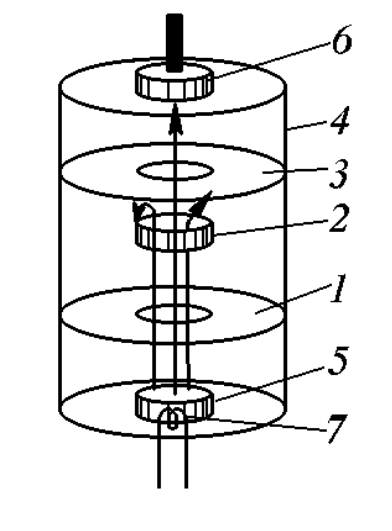
\includegraphics[width=0.6\linewidth]{Безымянный.png}
\caption{Схема тиратрона}
\label{fig:mpr}
\end{figure}

\begin{figure}[!h]
\centering
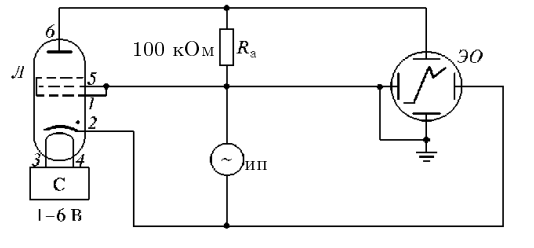
\includegraphics[width=0.8\linewidth]{Безымянный1.png}
\caption{Схема включения тиратрона}
\label{fig:mpr}
\end{figure}

Принципиальная схема установки для
изучения эффекта Рамзауэра приведена
на рис. 2. На лампу Л подаётся синусоидальное напряжение частоты 50 Гц от источника питания ИП, С — стабилизированный блок накала катода: исследуемый
сигнал подаётся на электронный осциллограф (ЭО); цифрами обозначены номера
ножек лампы.

Реально на экране ЭО удаётся надёжно наблюдать лишь один (первый, при $n=1$)
минимум в сечении рассеяния электронов и следующий за ним максимум .
Дело в том, что уже при $n=2$ напряжённость поля столь велика, что с большой вероятностью происходит ионизация атомов и возникает пробой тиратрона.

\paragraph{Ход работы и обработка результатов}

\subparagraph{1.}Для двух различных напряжений накала мы получили ВАХ в динамическом режиме на ЭО. Они изображены на Рис. 3 и Рис. 4.

\begin{figure}[!h]
\centering
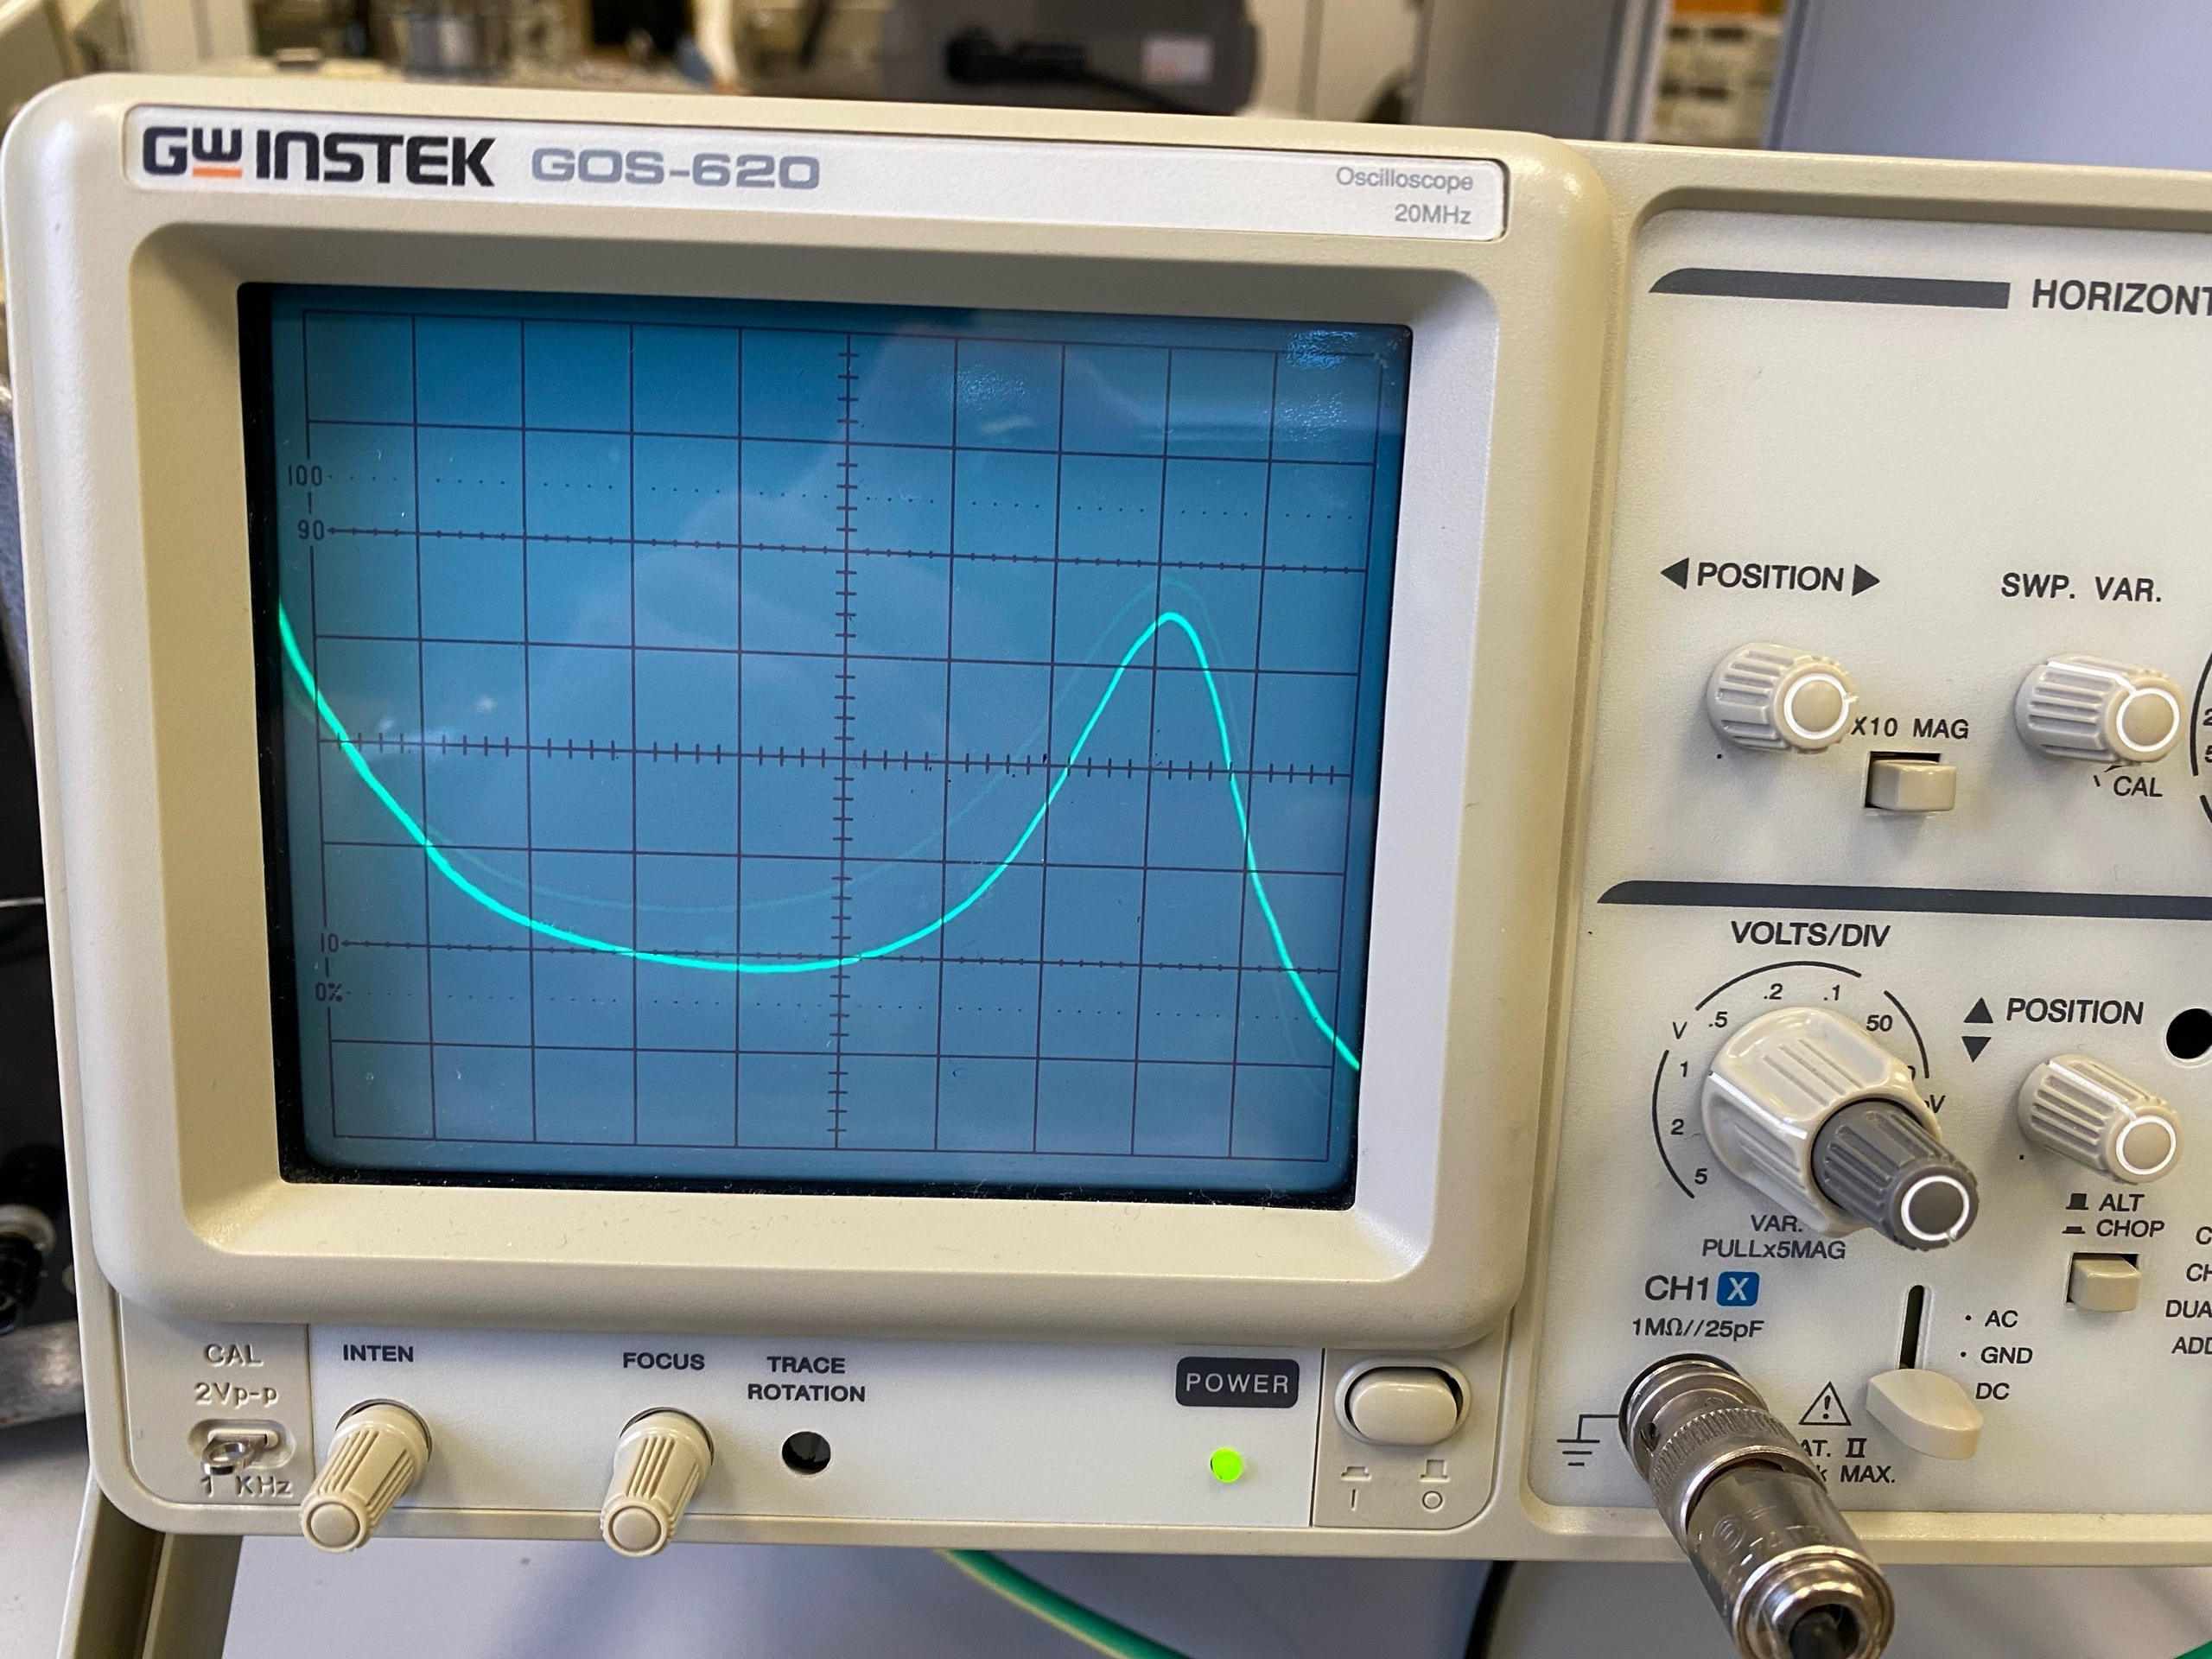
\includegraphics[width=0.7\linewidth]{cDMKSWgLqa4.jpg}
\caption{ВАХ для $U_{нак}=2,964$ В}
\label{fig:mpr}
\end{figure}

\begin{figure}[!h]
\centering
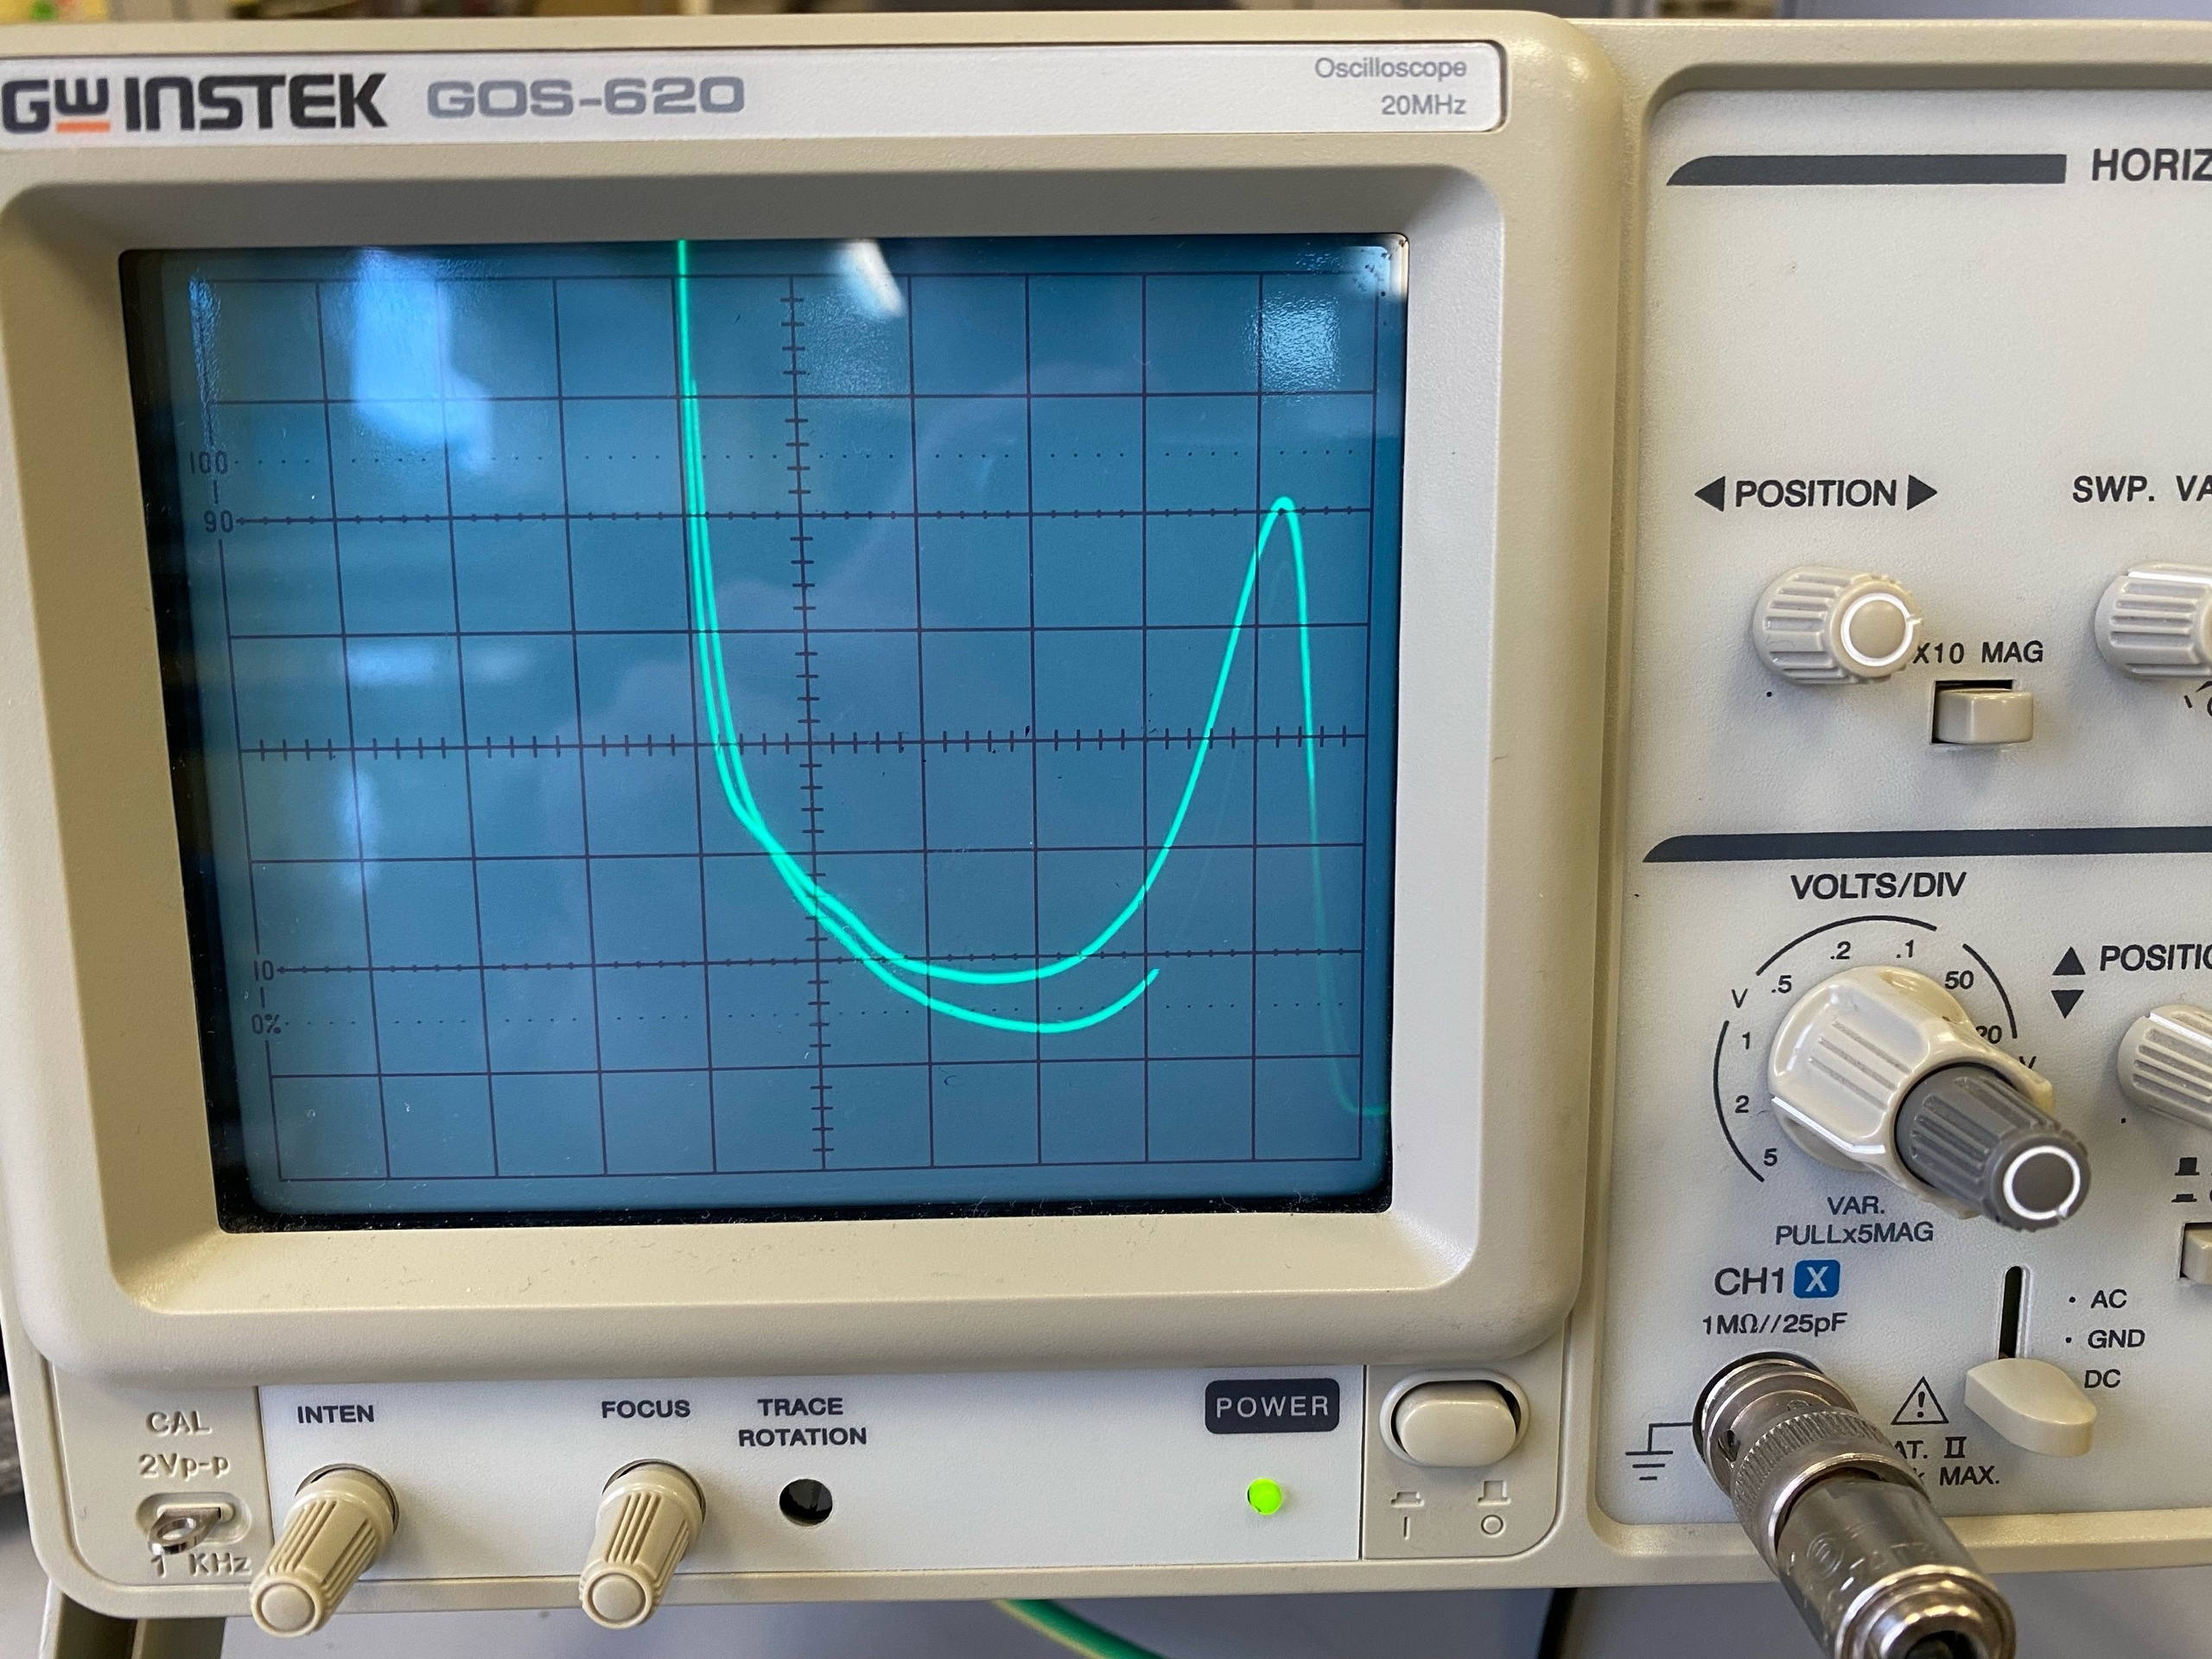
\includegraphics[width=0.7\linewidth]{XHpdd6O5oJE.jpg}
\caption{ВАХ для $U_{нак}=2,75$ В}
\label{fig:mpr}
\end{figure}

\subparagraph{2.}Затем в статическом режиме, изменяя напряжение на катоде, измеряли напряжение на аноде для двух токов накала. Зная сопротивление, легко получить ток. Результаты измерений приведены на Рис. 5 и Рис. 6.

\begin{figure}[!h]
\centering
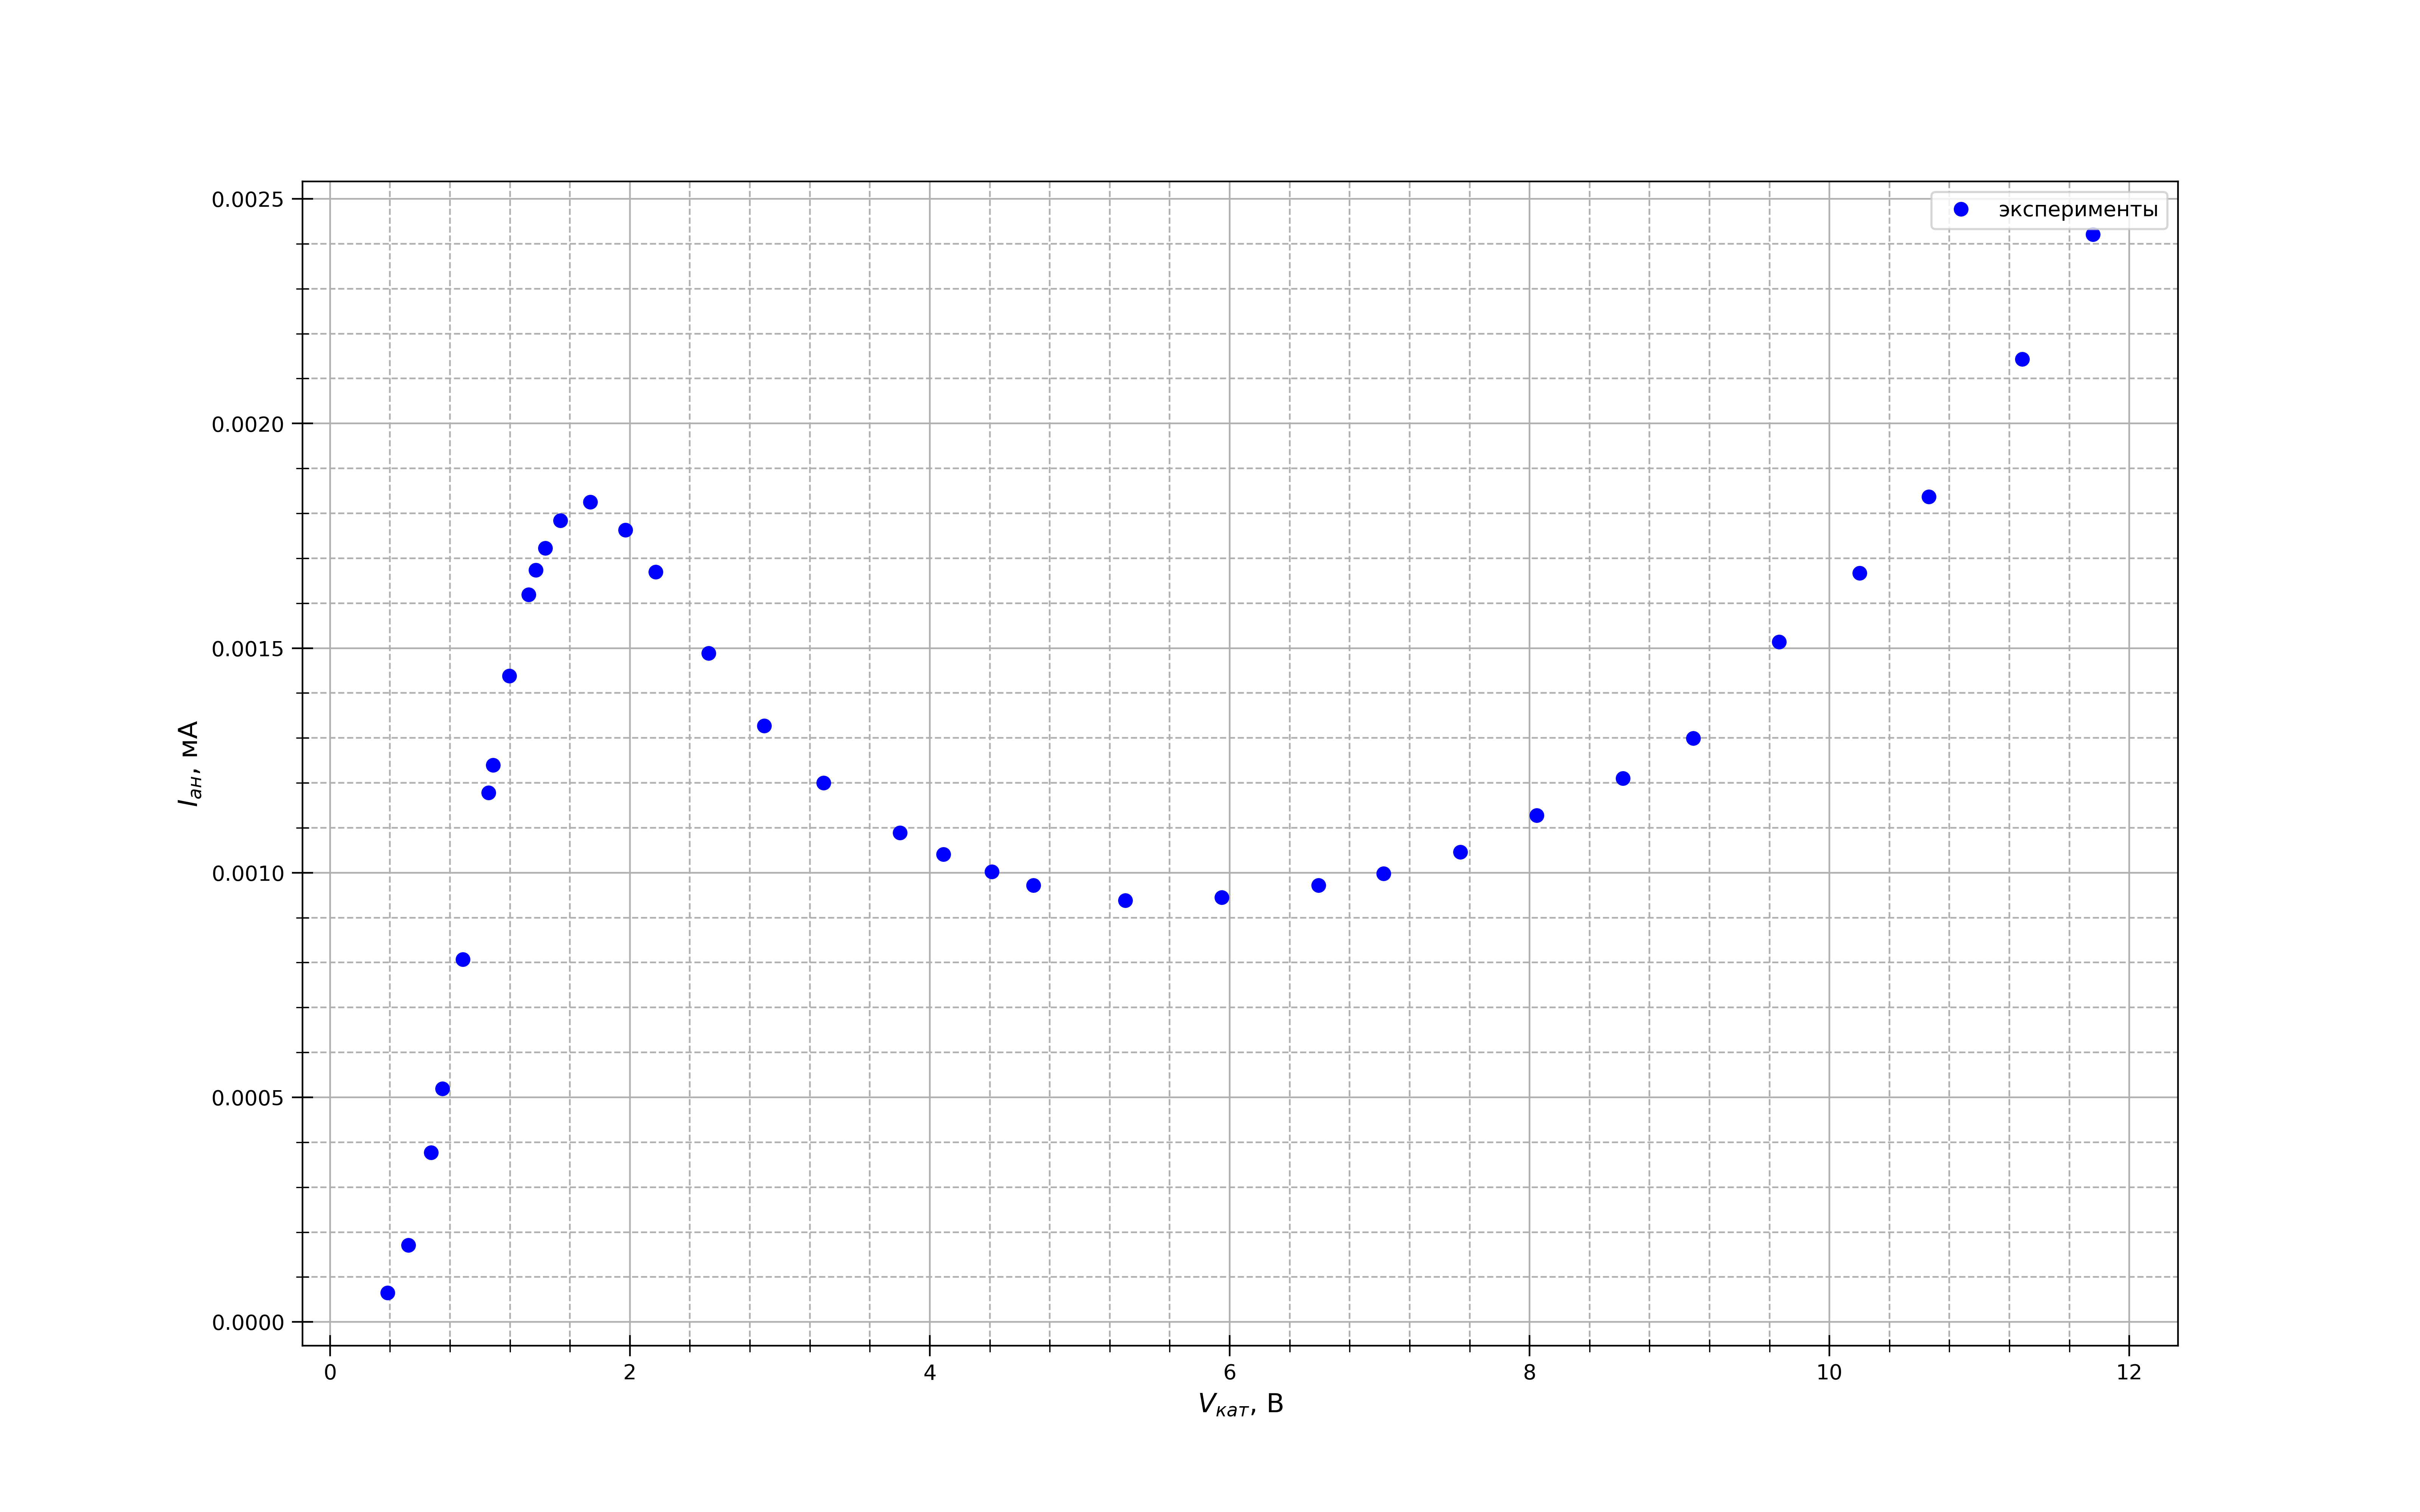
\includegraphics[width=0.8\linewidth]{nakal1.png}
\caption{ВАХ для $U_{нак}=2,964$ В}
\label{fig:mpr}
\end{figure}

\begin{figure}[!h]
\centering
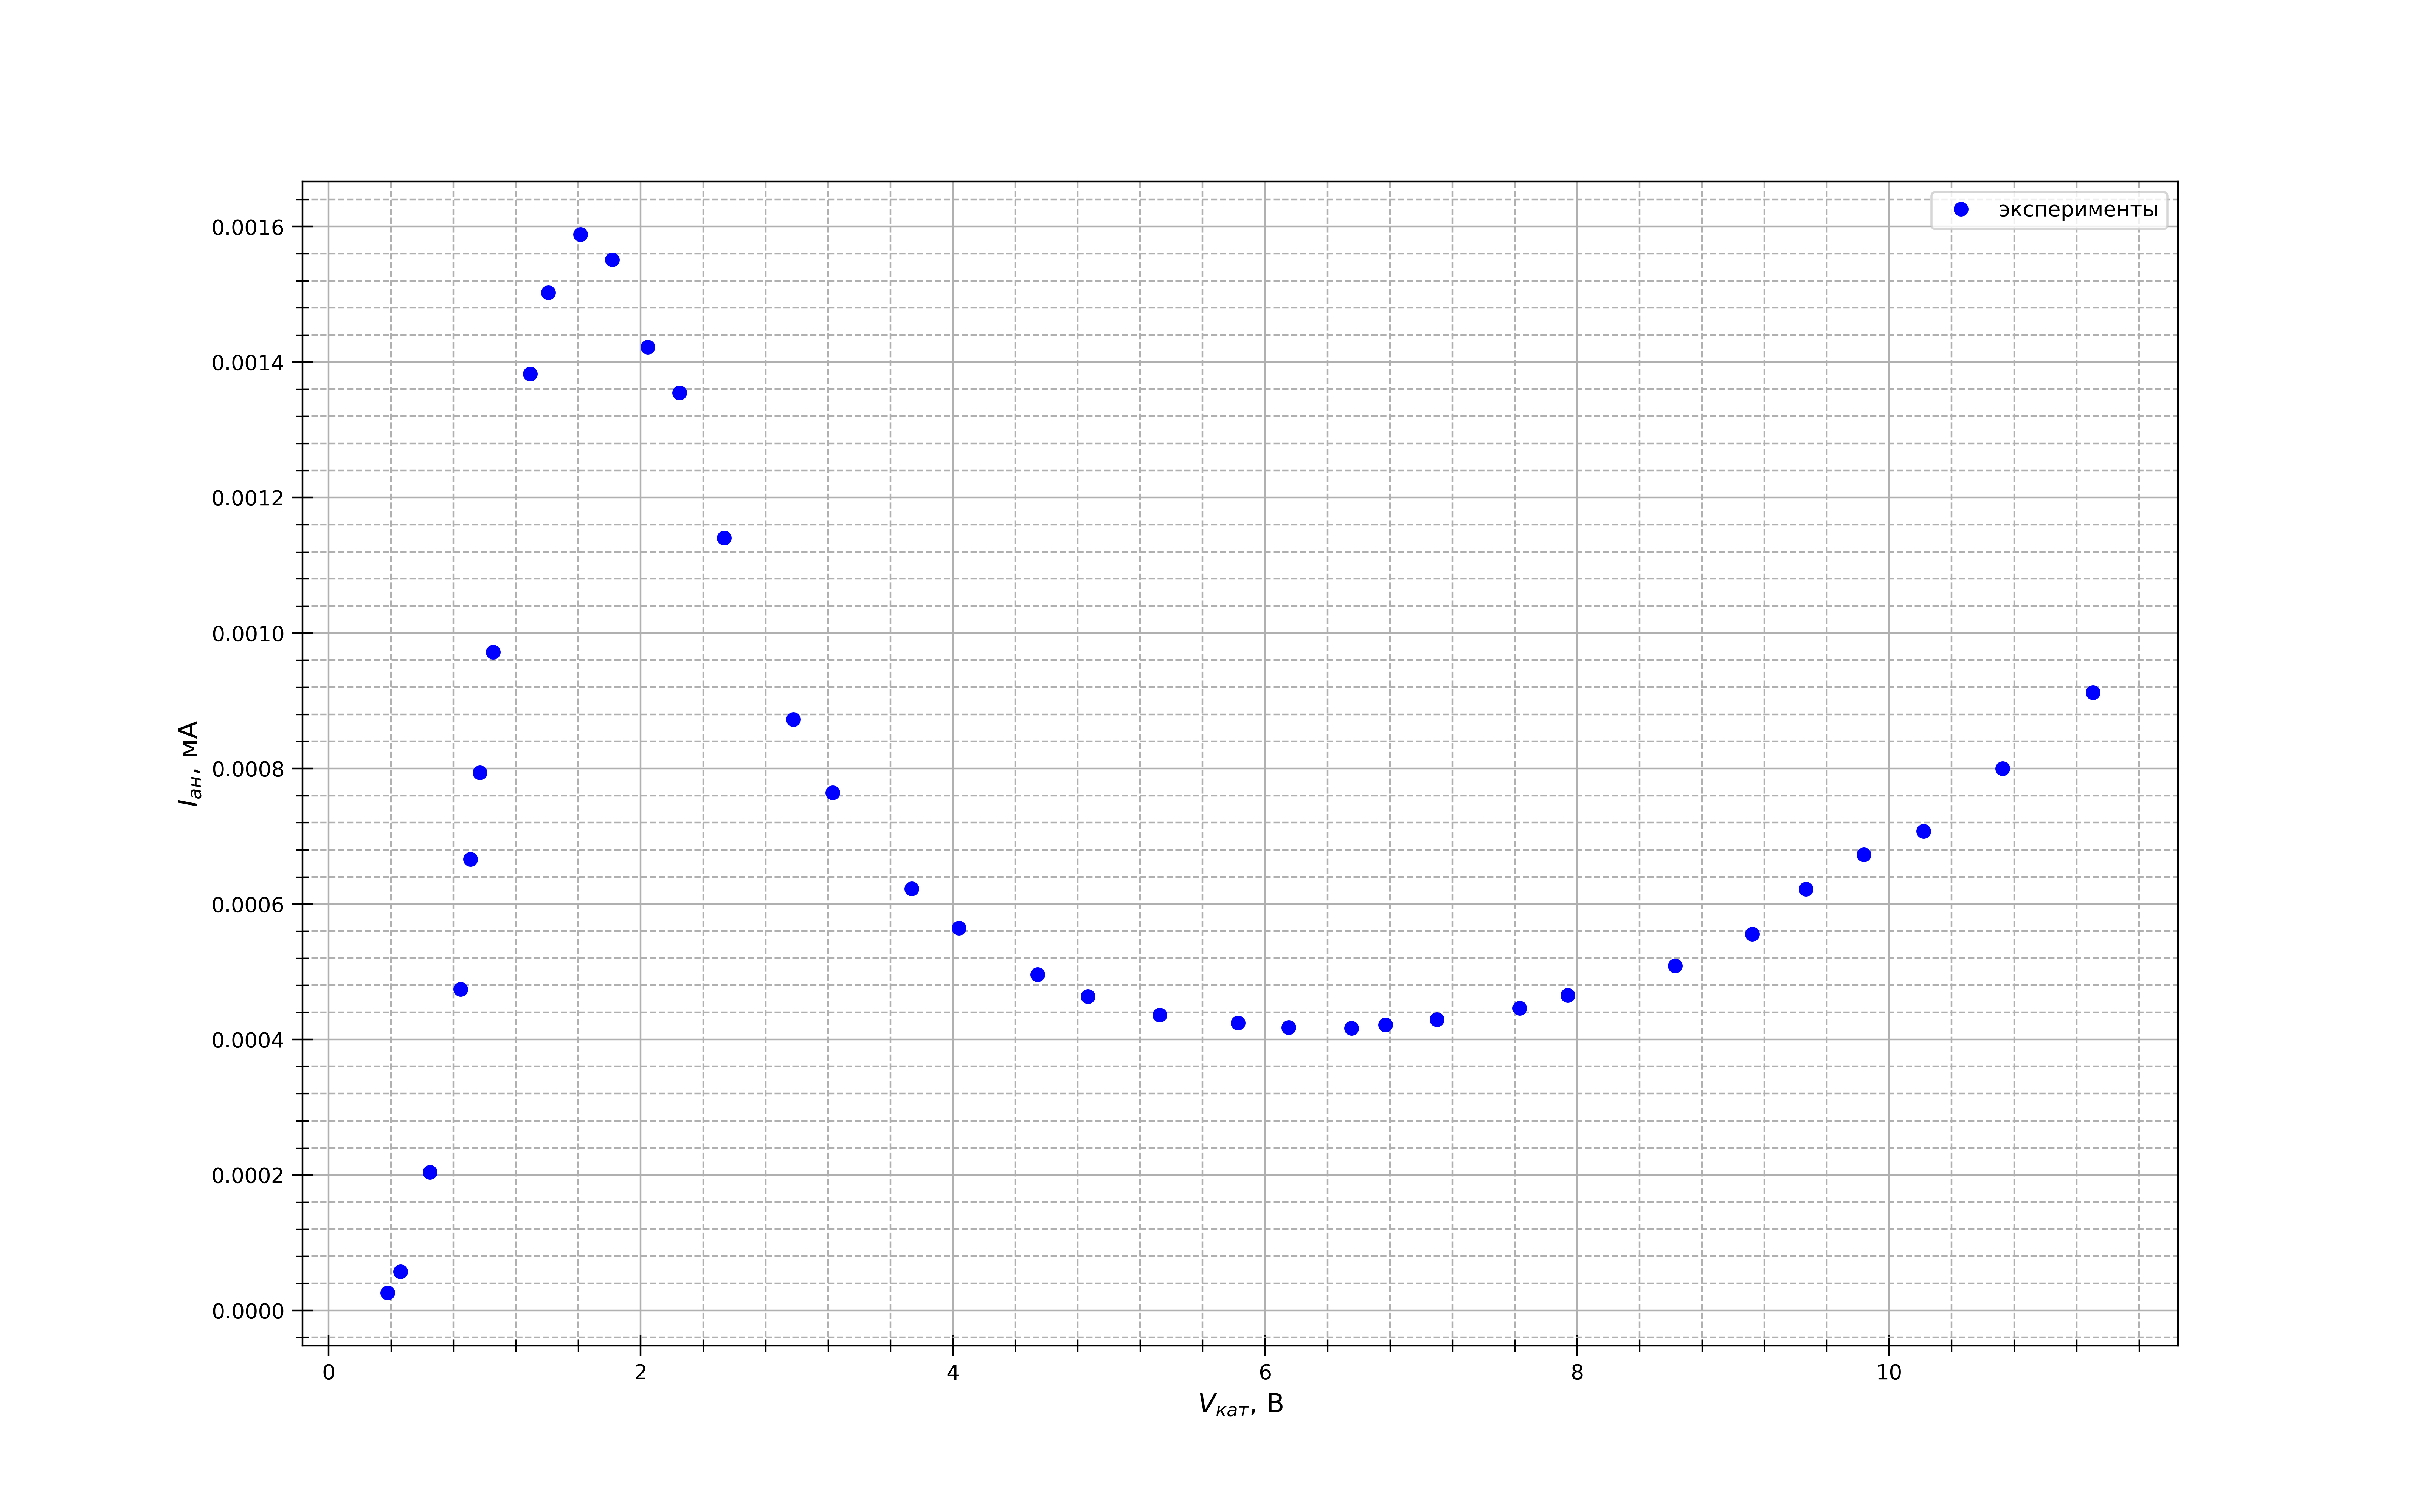
\includegraphics[width=0.8\linewidth]{nakal2.png}
\caption{ВАХ для $U_{нак}=2,75$ В}
\label{fig:mpr}
\end{figure}

\subparagraph{3.}Оценим размер атома газа. Примем $U_0=2,5$ В. Тогда по формуле $\sqrt{E_{light} + U_0 }[эВ] \frac{l}{1,95}[\textup{~\AA}]= \pi$ получаем:

\begin{center}
    $l = 2,95[\textup{~\AA}]$
\end{center}

Исключив $U_0$, по формуле $\sqrt{E_{dark} - E_{light}}[эВ] (\frac{l}{1,95}[\textup{~\AA}])^2= \frac{1}{4}\pi^2 + \pi^2$ получаем:

\begin{center}
    $l = 3,7[\textup{~\AA}]$
\end{center}

\subparagraph{4.} Разделив условия <<просветления>> и <<затемнения>> можно исключить размер ямы и выразить потенциальную глубину:

\begin{equation}
    U_0 = \frac{4}{5}E_{dark} - \frac{9}{5}E_{light} = 0,92 эВ
\end{equation}

\subparagraph{5.}Пробой тиратрона происходит приблизительно при 12 В, а ионизационный потенциал ксенона 12,1 эВ. Значит, в тиратроне ксенон. \par
Табличный размер атома ксенона 216 пм. Значения, получившиеся в предыдущих пунктах, близки.

\paragraph{Вывод:} в данной лабораторной работе мы исследовали ВАХ тиратрона. Из ВАХ нашли энергии <<просветления>> и <<затемнения>>, оценили размер атома инертного газа, глубину потенциальной ямы и определили газ в тиратроне.

\end{document}
